\documentclass{jsbook}
\usepackage[dvipdfmx]{graphicx}
\usepackage{comment}
\begin{document}
\chapter{最初の一歩}
	簡単な例を使ってCoqを使ってみる。
\newpage
%---------------------
\section{Coqを使ってみよう}
	\ref{準備}章ででインストールができたら実際にCoqを使ってみましょう。
	まず、どこかしらにインストールされた「CoqIde」を起動しましょう。
	
\begin{center}
	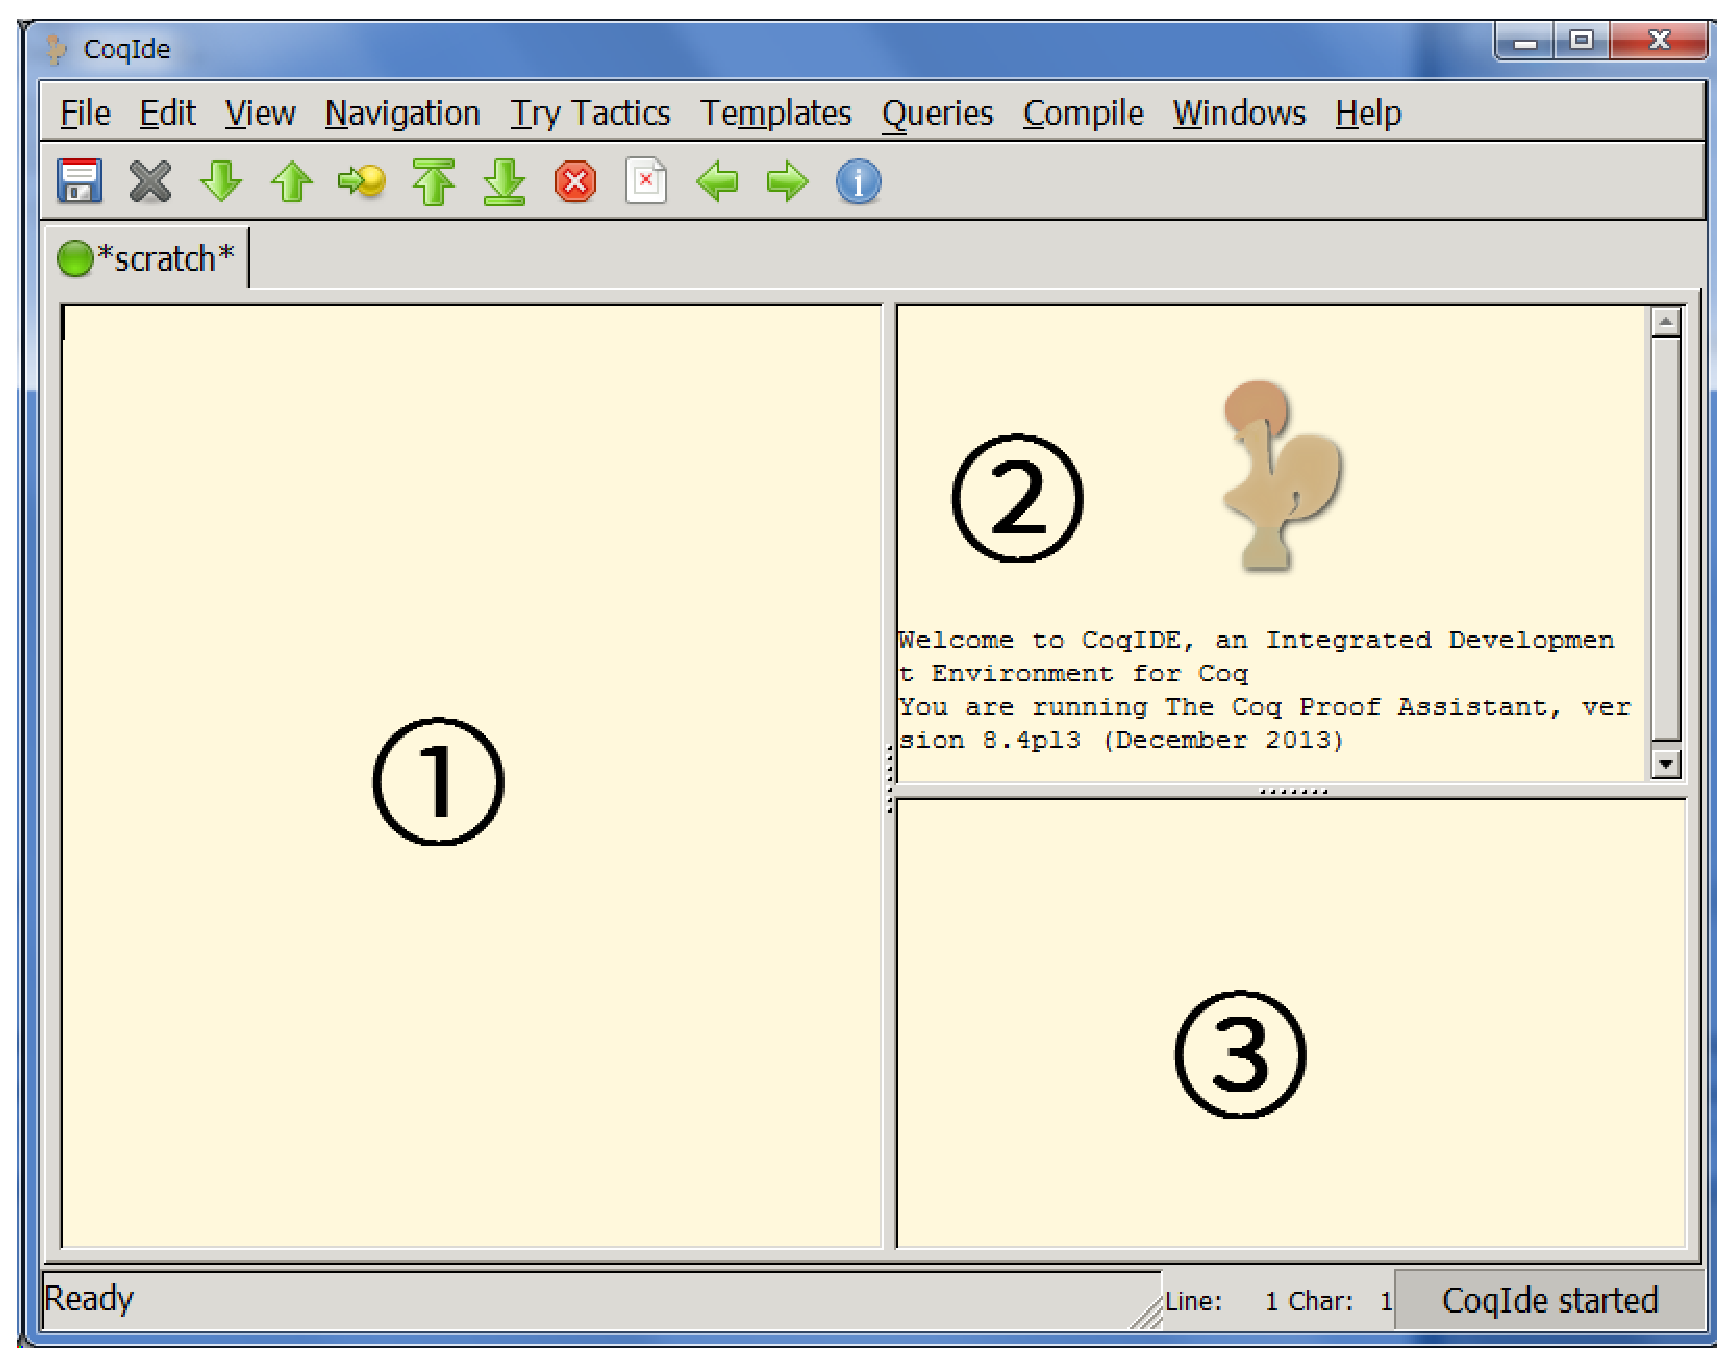
\includegraphics[width=38zw]{image/coqScrean.eps}\\
	\label{coqの画面}
\end{center}

上の画面がCoqIdeの画面です。
$ \textcircled{\footnotesize1} $がメインスペースです。ここに定義や定理、証明を記述していきます。
$ \textcircled{\footnotesize2} $は証明をするときに使います。証明の過程などが自動的に表示されます。
$ \textcircled{\footnotesize3} $はシステムメッセージの表示スペースです。

\subsection*{クエリペイン}
まず本当に簡単な例を使ってCoqの機能を使ってみましょう。
メニューバーのView から Show Query Paneをクリックするか、Escキーを押してください。
すると画面が変化して画面下から「Command Pane」が出てきます。
出てきたらそのペインの左にある3つアイコンの中から紙のようなアイコンをクリックします。
そうしたらペインの表示が変わって次の図のようになります。
\begin{center}
	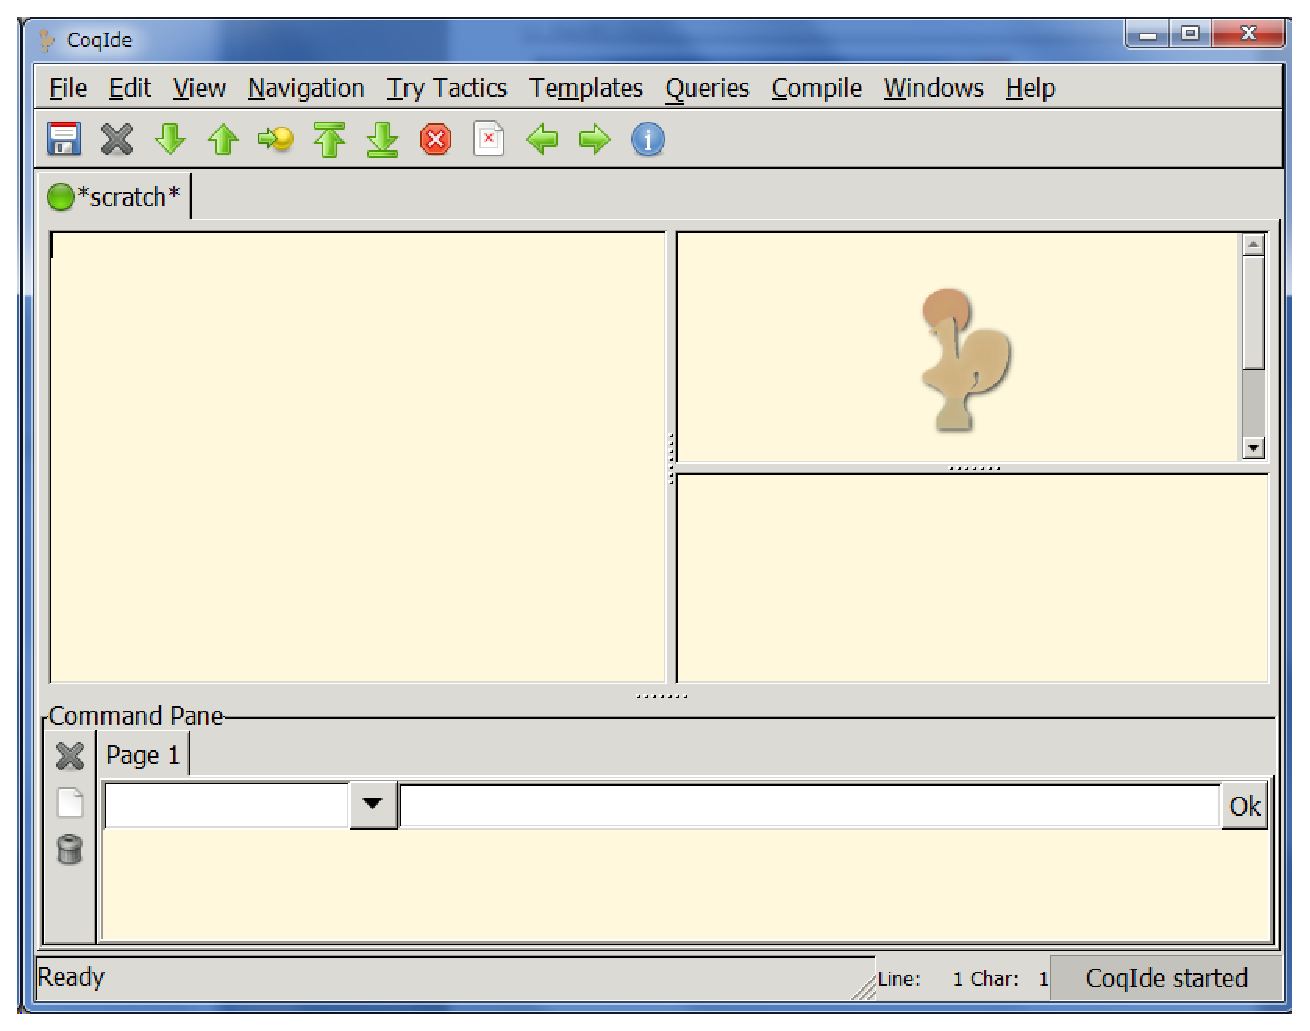
\includegraphics[width=38zw]{image/queryPane.eps}\\
	\label{querypane}
\end{center}

これでQuery Paneの使う準備が出来ました。
では早速使ってみましょう。
左のテキストボックスに「Eval compute in」を、右のテキストボックスに「3+4」と打ち込んでください。
Enterキーを押してペインの下側に
\begin{verbatim}
Result for command Eval compute in 3+4 . :
     = 7
     : nat
\end{verbatim}
と表示されればOKです。打ち込んだ通り、3+4の計算結果7が返されました。
これでQuery Paneを使えるようになりました。
え?これだけ?と思うかもしれませんが、\emph{今の時点では}これだけです。
あとで説明しますが、今ここでできることは自分で関数などを定義して読み込んだり、ライブラリを読み込むことでできることが増えていきます。
今の状態だとできるのは自然数の足し算・引き算・掛け算程度です。割り算や実数を扱った計算はできません。

今回は関数に自然数2つを入力し、帰ってきた結果を見ました。
このQuery Paneでは他にも様々なことが実行できます。
三角マークをクリックしてプルダウンリストを出すと、実行できるコマンドを見ることができます。
しかし、おそらく「Eval compute in」以外を使うことはほぼないと思います。

\begin{comment}
\section{節名未定}
ここでは、先ほど省略した部分を説明していきます。
説明したとおり、Eval compute inでできることは「関数などを定義し読み込む。もしくは、ライブラリを読み込む」ことで増えていきます。
ここではライブラリの読み込みでできることを増やしてみましょう。
関数の場合は、実際に関数を定義するときに一緒に説明します。

ではライブラリを読み込んでブーリアン型を使えるようにしましょう。
メインスペースに「Require Import Bool.」と書き込んで、上のツールバーにある左から3番目の下向き矢印をクリックしてください。
今書き込んだところが緑背景になればライブラリの読み込みが完了し、Query Paneでもライブラリにある関数などが使えるようになりました。

読み込んだライブラリを実際に使ってみましょう。
Query Paneの右側に「andb true false」と入力してEnterキーを押してください。
\begin{verbatim}
Result for command Eval compute in andb true false . :
     = false
     : bool
\end{verbatim}
となれば正しく読み込みができてます。
\end{comment}
%----------------------
\end{document}